\documentclass[a4paper, oneside]{discothesis}

\usepackage[utf8]{inputenc}
\usepackage[T1]{fontenc}
\usepackage{algpseudocode}
\usepackage{algorithm}
\usepackage{mathtools}
\usepackage{subcaption}
\usepackage{tikz}
\usetikzlibrary{arrows.meta}


%%%%%%%%%%%%%%%%%%%%%%%%%%%%%%%%%%%%%%%%%%%%%%%%%%%%%%%%%%%%%%%%%%%%%%%%%%%%%%%%%%%%%%%%%%%%%%%%%
% DOCUMENT METADATA

\thesistype{Bachelor's Thesis} % Master's Thesis, Bachelor's Thesis, Semester Thesis, Group Project
\title{Practical Dynamic Directories}

\author{Silvan Mosberger}
\email{msilvan@student.ethz.ch}

\institute{Distributed Computing Group \\[2pt]
Computer Engineering and Networks Laboratory \\[2pt]
ETH Zürich}

\supervisors{András Papp, Pankaj Khanchandani\\[2pt] Prof.\ Dr.\ Roger Wattenhofer}

% Optionally, keywords and categories of the work can be shown (on the Abstract page)
\keywords{Arrow, Ivy, distributed directory, shared object}
\categories{Network algorithms}

\date{\today}

%%%%%%%%%%%%%%%%%%%%%%%%%%%%%%%%%%%%%%%%%%%%%%%%%%%%%%%%%%%%%%%%%%%%%%%%%%%%%%%%%%%%%%%%%%%%%%%%%

\begin{document}

\frontmatter % do not remove this line
\maketitle
\TODO{Better title?}

\cleardoublepage

\begin{acknowledgements}
I thank Lorem ipsum dolor sit amet, consetetur sadipscing elitr, sed diam nonumy eirmod tempor invidunt ut labore et dolore magna aliquyam erat, sed diam voluptua. At vero eos et accusam et justo duo dolores et ea rebum. Stet clita kasd gubergren, no sea takimata sanctus est Lorem ipsum dolor sit amet. Lorem ipsum dolor sit amet, consetetur sadipscing elitr, sed diam nonumy eirmod tempor invidunt ut labore et dolore magna aliquyam erat, sed diam voluptua. At vero eos et accusam et justo duo dolores et ea rebum. Stet clita kasd gubergren, no sea takimata sanctus est Lorem ipsum dolor sit amet.
\end{acknowledgements}


\begin{abstract}
The abstract should be short, stating what you did and what the most important result is.
Lorem ipsum dolor sit amet, consetetur sadipscing elitr, sed diam nonumy eirmod tempor invidunt ut labore et dolore magna aliquyam erat, sed diam voluptua. At vero eos et accusam et justo duo dolores et ea rebum. Stet clita kasd gubergren, no sea takimata sanctus est Lorem ipsum dolor sit amet. Lorem ipsum dolor sit amet, consetetur sadipscing elitr, sed diam nonumy eirmod tempor invidunt ut labore et dolore magna aliquyam erat, sed diam voluptua. At vero eos et accusam et justo duo dolores et ea rebum. Stet clita kasd gubergren, no sea takimata sanctus est Lorem ipsum dolor sit amet.
\end{abstract}

\tableofcontents

\mainmatter

\chapter{Introduction}

Often in computing a single resource is shared between multiple components, where only one of them may access it at a time. In a distributed setting an algorithm to solve this is called a distributed mutual exclusion algorithm or distributed directory protocol. A trivial solution is to dedicate a single node to be the center where all requests for the resource should go, with the disadvantage of a lot of traffic for many concurrent requests. Better solutions to this problem include the Arrow and Ivy protocols, both of which work on similar principles to be explained in the following sections. In the Arvy paper these protocols have been combined in a flexible manner to allow a whole set of algorithms to be created while still guaranteeing correctness.

In this thesis we explore this set of Arvy algorithms with the hope of finding ones that work better than any already existing ones

\section{Model}

We consider a complete graph $G=(V,E)$ with $n\coloneqq|V|$ vertices and $m\coloneqq\binom{n}{2}$ edges. Each edge has a cost $c : E \rightarrow \mathbb{R}$ associated with it, representing the amount of time it takes a message to traverse it. The cost function forms a metric space:
\begin{itemize}
\item The cost from a node to itself is zero: $\forall v:c(v, v)=0$
\item Costs between different nodes are positive: $\forall u,v : u\neq v\Rightarrow c(u,v)>0$
\item Costs are the same in both directions: $\forall u,v : c(u,v)=c(v,u)$
\item Triangle inequality: $\forall u,v,w : c(u,w)\leq c(u,v)+c(v,w)$
\end{itemize}

As a reasonable constraint, a node $v$ can only query costs from itself to other nodes, so it has access to $\{c(v, u)\;|\;u\in V\}$. In a realistic scenario these costs can be obtained and updated by doing regular pings to other nodes. In our model we don't consider changing costs however.

In addition, Every node can be considered a machine with the ability to execute arbitrary effectful code such as reading/writing state or generating randomness. However execution is instantaneous, so no time passes during execution. Therefore traversing graph edges are the only place to spend time on.

A major simplification we make is that nodes can only request the token in series. So only after the token has reached the requesting node another node can make a request for it. Therefore requests can be represented as an series $r=\{r_i\},r_i\in N$ where $r_i$ encodes the $i$-th request originating from node $r_i$. For being able to reason more easily about execution time we let $i\in[1,i_{max}]$ to only have finitely many requests.

In the type of algorithms we'll look at, when the $i$-th request gets made by node $r_i$, the request travels along some path $p_i=\{p_{i0},p_{i1},\dots,p_{ip_{max}}\}$ of $p_{max}+1$ nodes \TODO{$p_{max}$ should really be ${p_{max}}_i$, better variable names?}, where $p_{i0}=r_i$ is the node making the request and $p_{ip_{max}}$ is the node currently holding the token. The token is then sent directly from $p_{ip_{max}}$ to $p_{i0}$ to satisfy the request. Without loss of generality, nodes can't send requests when they have the token already, meaning $p_{i0}\neq p_{ip_{max}}$.

The goal is to satisfy the requests most efficiently. We first define $\mathcal{C}(p_i)$ to be the cost of traversing path $p_i$:
\begin{equation}
\mathcal{C}(p_i)\coloneqq\sum_{k=1}^{p_{max}}c(p_{i(k-1)}, p_{ik})
\end{equation}

There are different ways to define efficiency in this context:
\begin{itemize}
\item
  One way is to look at the average time it takes to satisfy a request. This would include the cost to traverse the request path in addition to sending the token back. However because the cost to send the token back is unchangeable in our case we ignore it. Therefore
  \begin{equation}
    \mathcal{C}_{time}(r) = \frac{1}{i_{max}}\sum_i\mathcal{C}(p_i)
  \end{equation}

  This measure is better suited for overall performance because it reflects the average request.
  
\item
  Another way is to look at how much worse the request path is than how well it could have been by getting the ratio of the actual request path to what it could have been with a direct connection.
  \begin{equation}
    \mathcal{C}_{ratio}(r) = \frac{1}{i_{max}}\sum_i\frac{\mathcal{C}(p_i)}{c(p_{i0},p_{ip_{max}})}
  \end{equation}

  This measure penalizes request paths that are much longer than the direct path, so it's better suited for getting a sense of how individual requests are doing.

\item
  Even though in our model there is no execution time for computations on nodes, it could still be interesting to see how many nodes a request has to travel through. Therefore we define another measure, the average hop count:
  \begin{equation}
    \mathcal{C}_{hops}(r) = \frac{1}{i_{max}}\sum_ip_{max}
  \end{equation}
\end{itemize}

\section{Arrow, Ivy and Arvy}

Two well-known algorithms for solving this problem are Arrow and Ivy, which are both a special case of an Arvy algorithm, which is where its name comes from.

All of these algorithms are based on the idea of maintaining a rooted spanning tree over time: Every node stores a pointer to its parent $parent : V \rightarrow V$ while root nodes point to themselves. When a (non-root) node $a_0$ needs the token, it sends a request message towards its parent $a_1=parent(a_0)$. When a node $a_i$ receives such a request, it forwards it to $a_{i+1}=parent(a_i)$ and so on until the root $a_k$ containing the token is reached. This forms a request path $\{a_0,a_1,\dots,a_k\}$ of $k-1$ nodes. The final node then finishes its own work with the token after which it sends it directly to $a_0$. Now to make this a functioning algorithm, the arrows along this path need to be changed in some way such that the rooted tree is restored.

\subsection{Arrow}

The Arrow algorithm is the simplest way to maintain a rooted spanning tree, in that it just inverts the pointers along its path: When $a_{i+1}$ receives a request from $a_i$, it sets $parent(a_{i+1})=a_i$. See Figure~\ref{fig:arrow} for a walk-through of two requests with Arrow. Important on Arrow is that it doesn't ever change the structure of the spanning tree, meaning that the initial tree matters a lot for how well it performs.

\TODO{Bounds on Arrow}

\begin{figure}[]
\begin{subfigure}[t]{0.5\textwidth}
\centering
\begin{tikzpicture}
[bn/.style={circle,draw}
,root/.style={bn,thick}
,be/.style={draw=black,arrows={-Stealth[scale=1.5]}}
,req/.style={bn,red!70!black}
,auto,scale=0.7]
\node[root] (n1) at (0,5) {1};
\node[req] (n2) at (7,5) {2};
\node[above=0 of n2, red!70!black] {needs token};
\node[bn] (n3) at (3,4) {3};
\node[bn] (n4) at (2,1) {4};
\node[bn] (n5) at (6,0) {5};
\draw[be] (n2) -- (n3);
\draw[be] (n4) -- (n3);
\draw[be] (n5) -- (n4);
\draw[be] (n3) -- (n1);
\end{tikzpicture}
\caption{Node 2 needs the token}
\end{subfigure}
\quad
\begin{subfigure}[t]{0.5\textwidth}
\centering
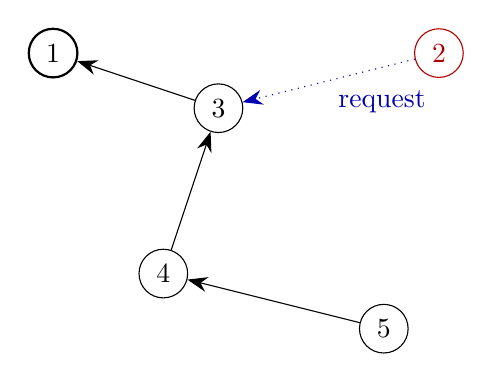
\begin{tikzpicture}
[bn/.style={circle,draw}
,root/.style={bn,thick}
,be/.style={draw=black,arrows={-Stealth[scale=1.5]}}
,req/.style={bn,red!70!black}
,auto,scale=0.7]
\node[root] (n1) at (0,5) {1};
\node[req] (n2) at (7,5) {2};
\node[bn] (n3) at (3,4) {3};
\node[bn] (n4) at (2,1) {4};
\node[bn] (n5) at (6,0) {5};
\draw[be] (n4) -- (n3);
\draw[be] (n5) -- (n4);
\draw[be] (n3) -- (n1);
\draw[be,dotted,blue!70!black] (n2) -- node{request} (n3);
\end{tikzpicture}
\caption{Node 2 sends a request towards its parent after which it sets its parent to itself to become a root}
\end{subfigure}

\begin{subfigure}[t]{0.5\textwidth}
\centering
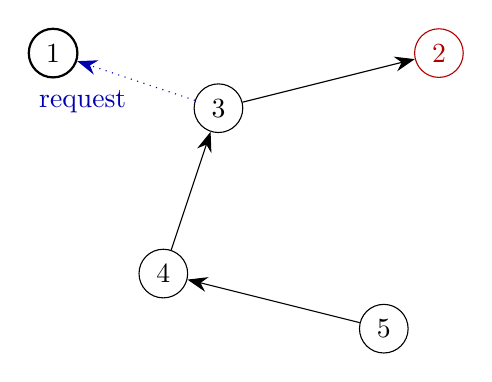
\begin{tikzpicture}
[bn/.style={circle,draw}
,root/.style={bn,thick}
,be/.style={draw=black,arrows={-Stealth[scale=1.5]}}
,req/.style={bn,red!70!black}
,auto,scale=0.7]
\node[root] (n1) at (0,5) {1};
\node[req] (n2) at (7,5) {2};
\node[bn] (n3) at (3,4) {3};
\node[bn] (n4) at (2,1) {4};
\node[bn] (n5) at (6,0) {5};
\draw[be] (n4) -- (n3);
\draw[be] (n5) -- (n4);
\draw[be] (n3) -- (n2);
\draw[be,dotted,blue!70!black] (n3) -- node{request} (n1);
\end{tikzpicture}
\caption{Node 3 receives the request and forwards it to its parent while changing its parent to the node it received the request from}
\end{subfigure}
\quad
\begin{subfigure}[t]{0.5\textwidth}
\centering
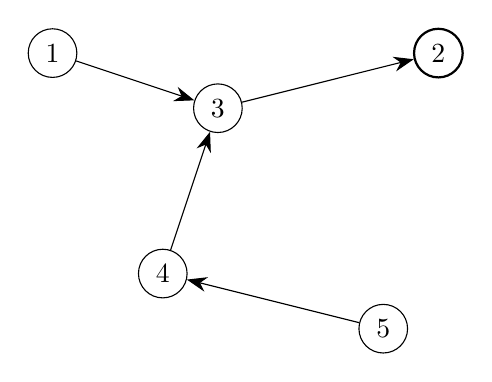
\begin{tikzpicture}
[bn/.style={circle,draw}
,root/.style={bn,thick}
,be/.style={draw=black,arrows={-Stealth[scale=1.5]}}
,req/.style={bn,red!70!black}
,auto,scale=0.7]
\node[bn] (n1) at (0,5) {1};
\node[root] (n2) at (7,5) {2};
\node[bn] (n3) at (3,4) {3};
\node[bn] (n4) at (2,1) {4};
\node[bn] (n5) at (6,0) {5};
\draw[be] (n4) -- (n3);
\draw[be] (n5) -- (n4);
\draw[be] (n3) -- (n2);
\draw[be] (n1) -- (n3);
\end{tikzpicture}
\caption{Node 1 which has the token receives the request, it sends the token to 2, making it the new root. It sets its parent to the node it received the request from}
\end{subfigure}

\begin{subfigure}[t]{0.5\textwidth}
\centering
\begin{tikzpicture}
[bn/.style={circle,draw}
,root/.style={bn,thick}
,be/.style={draw=black,arrows={-Stealth[scale=1.5]}}
,req/.style={bn,red!70!black}
,auto,scale=0.7]
\node[bn] (n1) at (0,5) {1};
\node[root] (n2) at (7,5) {2};
\node[bn] (n3) at (3,4) {3};
\node[bn] (n4) at (2,1) {4};
\node[req] (n5) at (6,0) {5};
\node[above=0 of n5, red!70!black] {needs token};
\draw[be] (n4) -- (n3);
\draw[be] (n5) -- (n4);
\draw[be] (n3) -- (n2);
\draw[be] (n1) -- (n3);
\draw[be,dotted,blue!70!black] (n5) .. controls (n4) and (n3) .. node[right]{request} (n2);
\end{tikzpicture}
\caption{Node 5 needs the token, resulting in a request path over $\{5,4,3,2\}$}
\end{subfigure}
\quad
\begin{subfigure}[t]{0.5\textwidth}
\centering
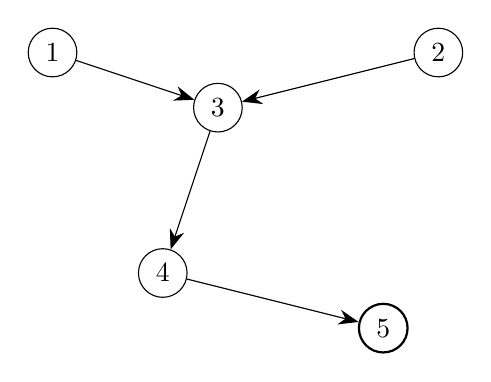
\begin{tikzpicture}
[bn/.style={circle,draw}
,root/.style={bn,thick}
,be/.style={draw=black,arrows={-Stealth[scale=1.5]}}
,req/.style={bn,red!70!black}
,auto,scale=0.7]
\node[bn] (n1) at (0,5) {1};
\node[bn] (n2) at (7,5) {2};
\node[bn] (n3) at (3,4) {3};
\node[bn] (n4) at (2,1) {4};
\node[root] (n5) at (6,0) {5};
\draw[be] (n2) -- (n3);
\draw[be] (n4) -- (n5);
\draw[be] (n3) -- (n4);
\draw[be] (n1) -- (n3);
\end{tikzpicture}
\caption{After node 2 with the token received the request it sent it to node 5. The nodes 4, 3 and 2 on the request path inverted the direction of their arrows}
\end{subfigure}
\caption{Arrow example}
\label{fig:arrow}
\end{figure}

\TODO{Abstract drawing stuff, perhaps implement Arvy in \LaTeX?}

\subsection{Ivy}

Ivy encompasses an entirely different way to invert the arrows along the request path, namely that every node $a_{i+1}$ receiving the request sets its parent to the node that made the request: $parent(a_{i+1})=a_0$. Therefore $a_0$ ends up being the center of a star consisting of all nodes along the request path.

\begin{figure}[]
\begin{subfigure}[t]{0.5\textwidth}
\centering
\begin{tikzpicture}
[bn/.style={circle,draw}
,root/.style={bn,thick}
,be/.style={draw=black,arrows={-Stealth[scale=1.5]}}
,req/.style={bn,red!70!black}
,auto,scale=0.7]
\node[root] (n1) at (0,5) {1};
\node[req] (n2) at (7,5) {2};
\node[above=0 of n2, red!70!black] {needs token};
\node[bn] (n3) at (3,4) {3};
\node[bn] (n4) at (2,1) {4};
\node[bn] (n5) at (6,0) {5};
\draw[be] (n2) -- (n3);
\draw[be] (n4) -- (n3);
\draw[be] (n5) -- (n4);
\draw[be] (n3) -- (n1);
\end{tikzpicture}
\caption{Node 2 needs the token}
\end{subfigure}
\quad
\begin{subfigure}[t]{0.5\textwidth}
\centering
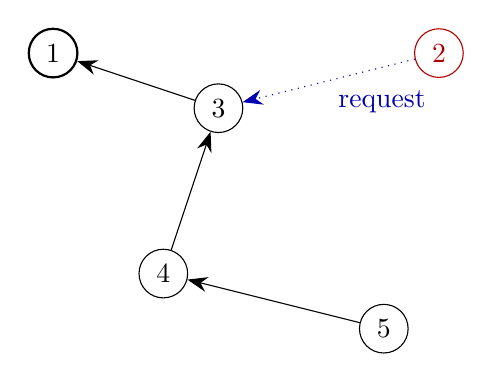
\begin{tikzpicture}
[bn/.style={circle,draw}
,root/.style={bn,thick}
,be/.style={draw=black,arrows={-Stealth[scale=1.5]}}
,req/.style={bn,red!70!black}
,auto,scale=0.7]
\node[root] (n1) at (0,5) {1};
\node[req] (n2) at (7,5) {2};
\node[bn] (n3) at (3,4) {3};
\node[bn] (n4) at (2,1) {4};
\node[bn] (n5) at (6,0) {5};
\draw[be] (n4) -- (n3);
\draw[be] (n5) -- (n4);
\draw[be] (n3) -- (n1);
\draw[be,dotted,blue!70!black] (n2) -- node{request} (n3);
\end{tikzpicture}
\caption{Node 2 sends a request towards its parent after which it sets its parent to itself to become a root}
\end{subfigure}

\begin{subfigure}[t]{0.5\textwidth}
\centering
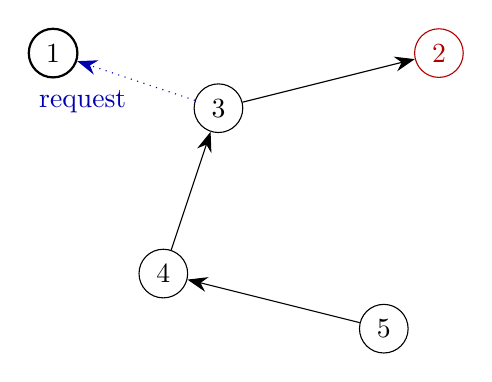
\begin{tikzpicture}
[bn/.style={circle,draw}
,root/.style={bn,thick}
,be/.style={draw=black,arrows={-Stealth[scale=1.5]}}
,req/.style={bn,red!70!black}
,auto,scale=0.7]
\node[root] (n1) at (0,5) {1};
\node[req] (n2) at (7,5) {2};
\node[bn] (n3) at (3,4) {3};
\node[bn] (n4) at (2,1) {4};
\node[bn] (n5) at (6,0) {5};
\draw[be] (n4) -- (n3);
\draw[be] (n5) -- (n4);
\draw[be] (n3) -- (n2);
\draw[be,dotted,blue!70!black] (n3) -- node{request} (n1);
\end{tikzpicture}
\caption{Node 3 receives the request and forwards it to its parent while changing its parent to the node that sent out the initial request}
\end{subfigure}
\quad
\begin{subfigure}[t]{0.5\textwidth}
\centering
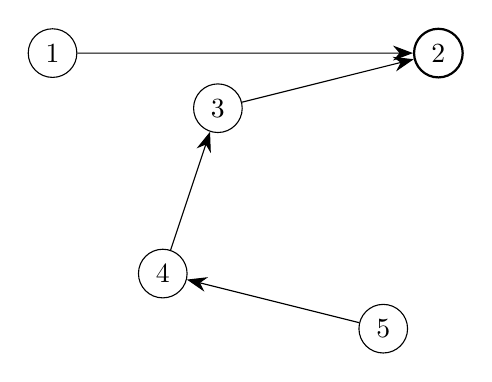
\begin{tikzpicture}
[bn/.style={circle,draw}
,root/.style={bn,thick}
,be/.style={draw=black,arrows={-Stealth[scale=1.5]}}
,req/.style={bn,red!70!black}
,auto,scale=0.7]
\node[bn] (n1) at (0,5) {1};
\node[root] (n2) at (7,5) {2};
\node[bn] (n3) at (3,4) {3};
\node[bn] (n4) at (2,1) {4};
\node[bn] (n5) at (6,0) {5};
\draw[be] (n4) -- (n3);
\draw[be] (n5) -- (n4);
\draw[be] (n3) -- (n2);
\draw[be] (n1) -- (n2);
\end{tikzpicture}
\caption{Node 1 which has the token receives the request, it sends the token to 2, making it the new root. It sets its parent to the node that sent out the initial request as well}
\end{subfigure}

\begin{subfigure}[t]{0.5\textwidth}
\centering
\begin{tikzpicture}
[bn/.style={circle,draw}
,root/.style={bn,thick}
,be/.style={draw=black,arrows={-Stealth[scale=1.5]}}
,req/.style={bn,red!70!black}
,auto,scale=0.7]
\node[bn] (n1) at (0,5) {1};
\node[root] (n2) at (7,5) {2};
\node[bn] (n3) at (3,4) {3};
\node[bn] (n4) at (2,1) {4};
\node[req] (n5) at (6,0) {5};
\node[above=0 of n5, red!70!black] {needs token};
\draw[be] (n4) -- (n3);
\draw[be] (n5) -- (n4);
\draw[be] (n3) -- (n2);
\draw[be] (n1) -- (n2);
\draw[be,dotted,blue!70!black] (n5) .. controls (n4) and (n3) .. node[right]{request} (n2);
\end{tikzpicture}
\caption{Node 5 needs the token, resulting in a request path over $\{5,4,3,2\}$}
\end{subfigure}
\quad
\begin{subfigure}[t]{0.5\textwidth}
\centering
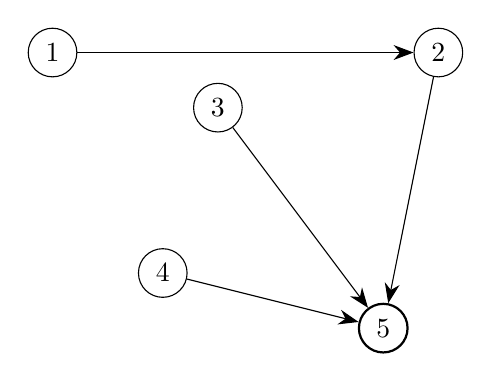
\begin{tikzpicture}
[bn/.style={circle,draw}
,root/.style={bn,thick}
,be/.style={draw=black,arrows={-Stealth[scale=1.5]}}
,req/.style={bn,red!70!black}
,auto,scale=0.7]
\node[bn] (n1) at (0,5) {1};
\node[bn] (n2) at (7,5) {2};
\node[bn] (n3) at (3,4) {3};
\node[bn] (n4) at (2,1) {4};
\node[root] (n5) at (6,0) {5};
\draw[be] (n2) -- (n5);
\draw[be] (n4) -- (n5);
\draw[be] (n3) -- (n5);
\draw[be] (n1) -- (n2);
\end{tikzpicture}
\caption{After node 2 with the token received the request it sent it to node 5. The nodes 4, 3 and 2 on the request path all set their parent to the node that sent out the initial request}
\end{subfigure}
\caption{Ivy example}
\label{fig:ivy}
\end{figure}

\subsection{Arvy}

Arvy generalizes the ideas of Arrow and Ivy by allowing nodes $a_{i+1}$ that received a request to set their parent to any node the request already traveled through, so $parent(a_{i+1})\in\{a_0,\dots,a_i\}$.

It's easy to see that this algorithm maintains a spanning tree over time with sequential requests. However this also holds for concurrent requests as the Arvy paper~\cite{Arvy} shows. Perhaps by surprise this means that no matter what nodes choose as their new parents, it can't prevent the algorithm from being correct.


\begin{figure}[]
\begin{subfigure}[t]{0.5\textwidth}
\centering
\begin{tikzpicture}
[bn/.style={circle,draw}
,root/.style={bn,thick}
,be/.style={draw=black,arrows={-Stealth[scale=1.5]}}
,req/.style={bn,red!70!black}
,auto,scale=0.7]
\node[root] (n1) at (0,5) {1};
\node[req] (n2) at (7,5) {2};
\node[above=0 of n2, red!70!black] {needs token};
\node[bn] (n3) at (3,4) {3};
\node[bn] (n4) at (2,1) {4};
\node[bn] (n5) at (6,0) {5};
\draw[be] (n2) -- (n3);
\draw[be] (n4) -- (n3);
\draw[be] (n5) -- (n4);
\draw[be] (n3) -- (n1);
\end{tikzpicture}
\caption{Node 2 needs the token}
\end{subfigure}
\quad
\begin{subfigure}[t]{0.5\textwidth}
\centering
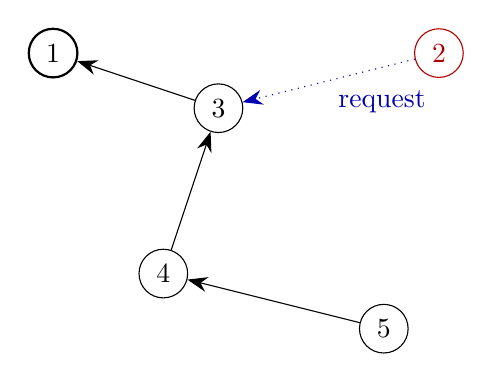
\begin{tikzpicture}
[bn/.style={circle,draw}
,root/.style={bn,thick}
,be/.style={draw=black,arrows={-Stealth[scale=1.5]}}
,req/.style={bn,red!70!black}
,auto,scale=0.7]
\node[root] (n1) at (0,5) {1};
\node[req] (n2) at (7,5) {2};
\node[bn] (n3) at (3,4) {3};
\node[bn] (n4) at (2,1) {4};
\node[bn] (n5) at (6,0) {5};
\draw[be] (n4) -- (n3);
\draw[be] (n5) -- (n4);
\draw[be] (n3) -- (n1);
\draw[be,dotted,blue!70!black] (n2) -- node{request} (n3);
\end{tikzpicture}
\caption{Node 2 sends a request towards its parent after which it sets its parent to itself}
\end{subfigure}

\begin{subfigure}[t]{0.5\textwidth}
\centering
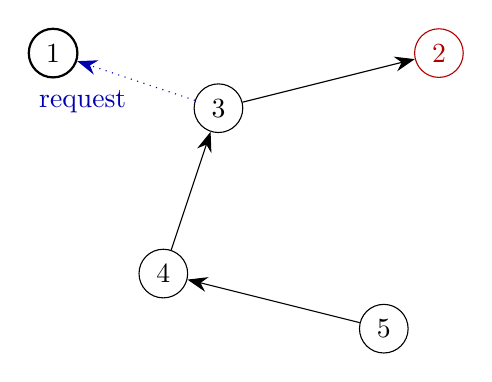
\begin{tikzpicture}
[bn/.style={circle,draw}
,root/.style={bn,thick}
,be/.style={draw=black,arrows={-Stealth[scale=1.5]}}
,req/.style={bn,red!70!black}
,auto,scale=0.7]
\node[root] (n1) at (0,5) {1};
\node[req] (n2) at (7,5) {2};
\node[bn] (n3) at (3,4) {3};
\node[bn] (n4) at (2,1) {4};
\node[bn] (n5) at (6,0) {5};
\draw[be] (n4) -- (n3);
\draw[be] (n5) -- (n4);
\draw[be] (n3) -- (n2);
\draw[be,dotted,blue!70!black] (n3) -- node{request} (n1);
\end{tikzpicture}
\caption{Node 3 receives the request and forwards it to its parent while changing its parent to the only previously visited node 2}
\end{subfigure}
\quad
\begin{subfigure}[t]{0.5\textwidth}
\centering
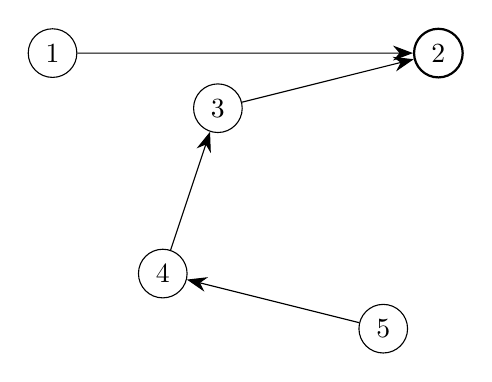
\begin{tikzpicture}
[bn/.style={circle,draw}
,root/.style={bn,thick}
,be/.style={draw=black,arrows={-Stealth[scale=1.5]}}
,req/.style={bn,red!70!black}
,auto,scale=0.7]
\node[bn] (n1) at (0,5) {1};
\node[root] (n2) at (7,5) {2};
\node[bn] (n3) at (3,4) {3};
\node[bn] (n4) at (2,1) {4};
\node[bn] (n5) at (6,0) {5};
\draw[be] (n4) -- (n3);
\draw[be] (n5) -- (n4);
\draw[be] (n3) -- (n2);
\draw[be] (n1) -- (n2);
\end{tikzpicture}
\caption{Node 1 which has the token receives the request, it sends the token to 2, making it the new root. Out of the possible new parents $\{2,3\}$ it chooses 2}
\end{subfigure}

\begin{subfigure}[t]{0.5\textwidth}
\centering
\begin{tikzpicture}
[bn/.style={circle,draw}
,root/.style={bn,thick}
,be/.style={draw=black,arrows={-Stealth[scale=1.5]}}
,req/.style={bn,red!70!black}
,auto,scale=0.7]
\node[bn] (n1) at (0,5) {1};
\node[root] (n2) at (7,5) {2};
\node[bn] (n3) at (3,4) {3};
\node[bn] (n4) at (2,1) {4};
\node[req] (n5) at (6,0) {5};
\node[above=0 of n5, red!70!black] {needs token};
\draw[be] (n4) -- (n3);
\draw[be] (n5) -- (n4);
\draw[be] (n3) -- (n2);
\draw[be] (n1) -- (n2);
\draw[be,dotted,blue!70!black] (n5) .. controls (n4) and (n3) .. node[right]{request} (n2);
\end{tikzpicture}
\caption{Node 5 needs the token, resulting in a request path over $\{5,4,3,2\}$}
\end{subfigure}
\quad
\begin{subfigure}[t]{0.5\textwidth}
\centering
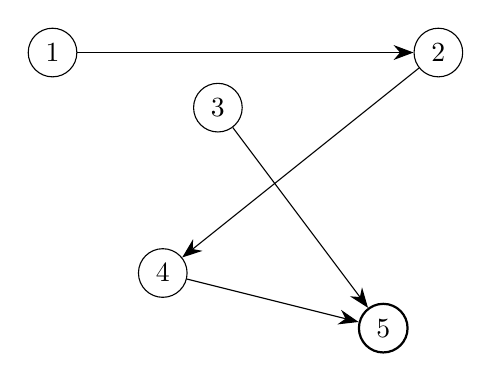
\begin{tikzpicture}
[bn/.style={circle,draw}
,root/.style={bn,thick}
,be/.style={draw=black,arrows={-Stealth[scale=1.5]}}
,req/.style={bn,red!70!black}
,auto,scale=0.7]
\node[bn] (n1) at (0,5) {1};
\node[bn] (n2) at (7,5) {2};
\node[bn] (n3) at (3,4) {3};
\node[bn] (n4) at (2,1) {4};
\node[root] (n5) at (6,0) {5};
\draw[be] (n2) -- (n4);
\draw[be] (n4) -- (n5);
\draw[be] (n3) -- (n5);
\draw[be] (n1) -- (n2);
\end{tikzpicture}
\caption{After node 2 with the token received the request it sent it to node 5. The nodes 4, 3 and 2 on the request path were able to choose its new parent from $\{5\}$, $\{5,4\}$ and $\{5,4,3\}$ respectively.}
\end{subfigure}
\caption{Arvy example}
\end{figure}


\chapter{Algorithms}

\begin{algorithm}
\caption{Arvy algorithm}
\label{test}
\begin{algorithmic}

\Function{RequestToken}{$a_0$}
\If{$parent(a_0)\neq a_0$}
    \State send request for token to $parent(a_0)$
    \State $parent(a_0)\gets a_0$
\EndIf
\EndFunction
\Function{ReceiveRequest}{$a_k$}
\If{$parent(a_k)=a_k$}
    \State send token to $a_0$
\Else
    \State forward request to $parent(a_k)$
\EndIf
\State $parent(a_k)\gets\;$\Call{SelectNewParent}{$a_0, a_1, \dots, a_{k-1}$}
\EndFunction
\Function{SelectNewParent}{$\{a_i\}$}
\State\Return any of $a_i$
\EndFunction
\end{algorithmic}
\end{algorithm}


\section{Arrow}

Arrow is a specialized version of Arvy that makes nodes along the request path always select the most recent node as a new parent
\begin{algorithmic}
\Function{SelectNewParent}{$\{a_i\}$}
\State\Return $a_i$
\EndFunction
\end{algorithmic}

\section{Ivy}

Similarly, Ivy is a specialized version of Arvy that makes nodes along the request path always select the oldest node as a new parent, which is always the node that made the request originally
\begin{algorithmic}
\Function{SelectNewParent}{$\{a_i\}$}
\State\Return $a_0$
\EndFunction
\end{algorithmic}

\chapter{Results}

Should include
\begin{itemize}
\item Resulting plots of interesting evaluations
\item Show how to reproduce the results including parameters
\end{itemize}

\chapter{Program Design}

Should include
\begin{itemize}
\item How the program design only allows expressing valid Arvy algorithms
\end{itemize}


\begin{theorem}[First Theorem]\label{thm:first theorem}
	This is our first theorem.
\end{theorem}

\begin{proof}
	And this is the proof of the first theorem with a complicated formula and a reference to Theorem \ref{thm:first theorem}. Lorem ipsum dolor sit amet, consetetur sadipscing elitr, sed diam nonumy eirmod tempor invidunt ut labore et dolore magna aliquyam erat, sed diam voluptua. Lorem ipsum dolor sit amet, consetetur sadipscing elitr, sed diam nonumy eirmod tempor invidunt ut labore et dolore magna aliquyam erat, sed diam voluptua.
	\begin{equation}
		{\frac {\mathrm d}{\mathrm dx}}\arctan(\sin({x}^{2}))=-2 \cdot {\frac {\cos({x}^{2})x}{-2+\left (\cos({x}^{2})\right )^{2}}}
	\end{equation}	
\end{proof}

\begin{figure}
    \centering
    
\includegraphics[width=0.2\columnwidth]{figures/disco_logo_faded}
    \caption{This is an example graphic.}
    \label{fig:example_figure}
\end{figure}

And here we cite some external documents~\cite{TestReference, TestReference2}.
An example of an included graphic can be found in Figure~\ref{fig:example_figure}.
Note that in \LaTeX, ``quotes'' do not use the usual double quote characters.

% This displays the bibliography for all cited external documents. All references have to be defined in the file references.bib and can then be cited from within this document.
\bibliographystyle{IEEEtran}
\bibliography{references}

% This creates an appendix chapter, comment if not needed.
\appendix
\chapter{First Appendix Chapter Title}

\end{document}
